\documentclass[12pt]{article}
\usepackage[margin=1in]{geometry}
\usepackage{graphicx}
\usepackage{amsmath,amssymb,bm}
\usepackage{float}
\usepackage{caption}
\usepackage{setspace}
\usepackage{tikz}
\usepackage{xcolor}
\usepackage{algorithm}
\usepackage{algpseudocode}
\usepackage[hidelinks]{hyperref}
\captionsetup[algorithm]{labelformat=empty, name={}}
\usetikzlibrary{arrows.meta, calc, positioning}
\captionsetup{font=small, labelfont=bf, skip=6pt}
\onehalfspacing
\graphicspath{{figures/rnn_lstm/}{figures/}}

\definecolor{MITgreen}{HTML}{C0E0B0}
\definecolor{MITblue}{HTML}{B0D0E0}
\definecolor{MITpurple}{HTML}{D0B0F0}

\title{Recurrent Networks and LSTMs}
\author{Volatility forecasting project}
\date{1 October 2026}

\begin{document}
\maketitle

\noindent
Recurrent neural networks (RNNs) and long short-term memory (LSTM) cells process
sequences by carrying a state across time. This section states the recurrence,
the training failure modes of a plain RNN, and the gated LSTM update used later
for one-day-ahead \(\log\mathrm{RV}\) forecasting.

\section{Why recurrence}
A feed-forward net maps one input vector to one output.
A time series needs something else: the prediction at step \(t\) should depend on
what came before, not only on \(x_t\).

An RNN does that with a \emph{hidden state} \(h_t\) that is updated every step and
passed forward. The same parameters are reused at every \(t\).
In compact form,
\[
\hat y_t \;=\; f\!\bigl(x_t,\, h_{t-1}\bigr).
\]
\begin{figure}[H]
\centering
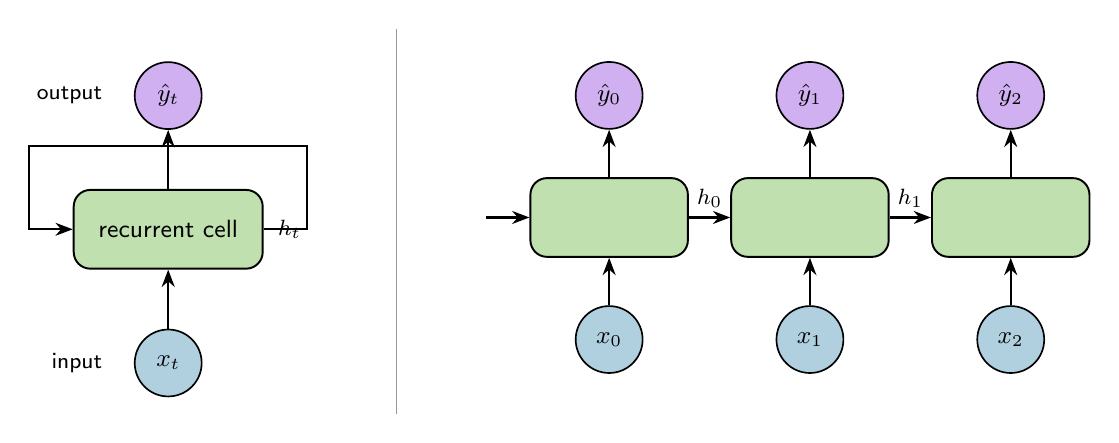
\begin{tikzpicture}[
  cell/.style={draw=black, fill=MITgreen, rounded corners=6pt,
               minimum width=2.4cm, minimum height=1.0cm,
               font=\sffamily\small, align=center, line width=0.7pt},
  ycirc/.style={circle, draw=black, fill=MITpurple, minimum size=0.85cm,
               inner sep=0pt, font=\small, line width=0.6pt},
  xcirc/.style={circle, draw=black, fill=MITblue, minimum size=0.85cm,
               inner sep=0pt, font=\small, line width=0.6pt},
  arr/.style={-{Stealth[length=2.2mm]}, line width=0.75pt, black},
  ]
  \begin{scope}[shift={(0,0)}]
    \node[cell] (cellL) {recurrent cell};
    \node[ycirc, above=0.75cm of cellL] (yL) {$\hat{y}_t$};
    \node[xcirc, below=0.75cm of cellL] (xL) {$x_t$};
    \draw[arr] (cellL.north) -- (yL.south);
    \draw[arr] (xL.north) -- (cellL.south);
    \node[left=0.28cm of yL, font=\sffamily\footnotesize, anchor=east] {output};
    \node[left=0.28cm of xL, font=\sffamily\footnotesize, anchor=east] {input};
    \coordinate (rA) at ([xshift=0.55cm]cellL.east);
    \coordinate (rB) at ([xshift=0.55cm,yshift=0.55cm]cellL.north east);
    \coordinate (rC) at ([xshift=-0.55cm,yshift=0.55cm]cellL.north west);
    \coordinate (rD) at ([xshift=-0.55cm]cellL.west);
    \draw[line width=0.75pt, black, -{Stealth[length=2.2mm]}]
      (cellL.east) -- (rA) -- (rB) -- (rC) -- (rD) -- (cellL.west);
    \node[font=\footnotesize, anchor=west] at ([xshift=0.06cm]cellL.east) {$h_t$};
  \end{scope}
  \draw[black!40, line width=0.6pt] (2.9,-2.35) -- (2.9,2.55);
  \begin{scope}[shift={(5.6,0.15)}]
    \foreach \i/\labx/\laby in {0/$x_0$/$\hat{y}_0$, 1/$x_1$/$\hat{y}_1$, 2/$x_2$/$\hat{y}_2$} {
      \pgfmathsetmacro{\xpos}{\i*2.55}
      \node[cell, minimum width=2.0cm] (C\i) at (\xpos,0) {};
      \node[ycirc] (Y\i) at (\xpos,1.55) {\laby};
      \node[xcirc] (X\i) at (\xpos,-1.55) {\labx};
      \draw[arr] (C\i.north) -- (Y\i.south);
      \draw[arr] (X\i.north) -- (C\i.south);
    }
    \draw[arr] (C0.east) -- node[above, font=\footnotesize, pos=0.5] {$h_0$} (C1.west);
    \draw[arr] (C1.east) -- node[above, font=\footnotesize, pos=0.5] {$h_1$} (C2.west);
    \draw[arr] ([xshift=-0.55cm]C0.west) -- (C0.west);
  \end{scope}
\end{tikzpicture}
\caption{Recurrent cell (left) and the same recurrence over three time steps (right).}
\end{figure}

\section{A simple RNN cell}
The simplest recurrent unit applies one nonlinearity to the concatenated
current input and previous hidden state:
\[
h_t \;=\; \tanh\!\bigl(W\,[h_{t-1},\, x_t] + b\bigr).
\]
Everything that the network ``remembers'' must travel through that single path.
\begin{figure}[H]
\centering
\includegraphics[width=0.92\textwidth]{LSTM3-SimpleRNN.png}
\caption{Repeating RNN module~\cite{olah2015}. Inside \(A\): one \(\tanh\) layer.
\(h_t\) is both the output at \(t\) and the memory passed to \(t+1\).}
\end{figure}

\section{Problems of a plain RNN}
Training unrolls the recurrence over many steps (backpropagation through time).
The same weights are applied at every \(t\), so gradients are products of many
Jacobians. Two failure modes follow.

\noindent\textbf{Exploding gradients.}
If those products grow without bound, updates become unstable.
A standard fix is \emph{gradient clipping}: after the backward pass, shrink the
gradient vector when its norm exceeds a threshold \(\tau\).

\begin{algorithm}[H]
\caption{Algorithm. Gradient clipping}
\begin{algorithmic}
\State \(\mathbf{g} \gets \nabla_{\theta}\mathcal{L}\)
\If{\(\lVert\mathbf{g}\rVert > \tau\)}
  \State \(\mathbf{g} \gets \tau\,\mathbf{g}/\lVert\mathbf{g}\rVert\)
\EndIf
\State \(\theta \gets \theta - \eta\,\mathbf{g}\)
\end{algorithmic}
\end{algorithm}

Clipping controls the size of the step. It does not create a better path for
information to travel across time.

\noindent\textbf{Vanishing gradients.}
If the products shrink toward zero, early timesteps stop affecting the loss.
Weight updates then ignore long-range dependence even when it is present in the
data. Rescaling \(\mathbf{g}\) does not fix that: the signal from the distant past
is already gone. The usual remedy is architectural---a cell that can carry
state across many steps without repeatedly multiplying through a saturating
nonlinearity. That motivates the LSTM below.

\section{LSTM: a gated memory}
An LSTM keeps two signals at each step:
\begin{itemize}
  \item a \emph{cell state} \(c_t\) --- a slow path that can carry information across many steps with mostly linear updates;
  \item a \emph{hidden state} \(h_t\) --- the exposed summary used as output and as input to the next step.
\end{itemize}
Three sigmoid \emph{gates} (values in \((0,1)\)) control write / erase / read on the cell.
\begin{figure}[H]
\centering
\includegraphics[width=0.95\textwidth]{LSTM3-chain.png}\\[0.8em]
\includegraphics[width=0.72\textwidth]{LSTM2-notation.png}
\caption{LSTM chain~\cite{olah2015}. The top horizontal line is the cell state.
Gates (yellow \(\sigma\) / \(\tanh\) layers and pink pointwise ops) edit that line
at each step, then form \(h_t\).}
\end{figure}

\section{Gates, step by step}
On timestep \(t\), the network receives \(x^{(t)}\) and the previous pair
\(\bigl(h^{(t-1)},\, c^{(t-1)}\bigr)\), and produces
\(\bigl(h^{(t)},\, c^{(t)}\bigr)\):
\begin{align*}
\bm{f}^{(t)}
  &= \sigma\!\bigl(W_f\,\bm{h}^{(t-1)} + U_f\,\bm{x}^{(t)} + \bm{b}_f\bigr)
  && \text{forget gate} \\[4pt]
\bm{i}^{(t)}
  &= \sigma\!\bigl(W_i\,\bm{h}^{(t-1)} + U_i\,\bm{x}^{(t)} + \bm{b}_i\bigr)
  && \text{input gate} \\[4pt]
\bm{o}^{(t)}
  &= \sigma\!\bigl(W_o\,\bm{h}^{(t-1)} + U_o\,\bm{x}^{(t)} + \bm{b}_o\bigr)
  && \text{output gate} \\[4pt]
\tilde{\bm{c}}^{(t)}
  &= \tanh\!\bigl(W_c\,\bm{h}^{(t-1)} + U_c\,\bm{x}^{(t)} + \bm{b}_c\bigr)
  && \text{candidate content} \\[4pt]
\bm{c}^{(t)}
  &= \bm{f}^{(t)}\odot \bm{c}^{(t-1)} + \bm{i}^{(t)}\odot \tilde{\bm{c}}^{(t)}
  && \text{cell update} \\[4pt]
\bm{h}^{(t)}
  &= \bm{o}^{(t)}\odot \tanh\bm{c}^{(t)}
  && \text{hidden state}
\end{align*}

Forget scales the old cell (near \(0\) erases, near \(1\) keeps).
Input scales how much new candidate content is written.
Output chooses what of \(\tanh(c_t)\) becomes \(h_t\).
The cell update is almost additive: erase some of \(c_{t-1}\), add some of \(\tilde c_t\).
That additive path is what makes long-range gradients viable.

\begin{figure}[H]
\centering
\includegraphics[width=0.98\textwidth]{Stanford-CS224N-L6-slide24.png}
\caption{Annotated LSTM cell: forget, write, and read
on the cell state, then \(h_t\) (and an optional readout \(\hat y_t\)).}
\end{figure}

\section{Reading the cell diagram}
\begin{center}
\renewcommand{\arraystretch}{1.25}
\begin{tabular}{@{}ll@{}}
\hline
\textbf{Signal} & \textbf{Role} \\
\hline
Forget gate \(f_t\) &
  what to keep from \(c_{t-1}\) \\
Input gate \(i_t\) &
  what of \(\tilde c_t\) to write \\
Candidate \(\tilde c_t\) &
  new content proposed at \(t\) \\
Cell \(c_t\) &
  memory: forget then write \\
Output gate \(o_t\) &
  what of the cell to expose \\
Hidden \(h_t\) &
  output at \(t\); input to step \(t+1\) \\
\hline
\end{tabular}
\end{center}
\vspace{0.6em}

In a forecasting model the readout from \(h_t\) is usually a linear map to a scalar
(or a small head), not a softmax over a vocabulary.
The cell mechanics above are unchanged; only the final layer depends on the task.

\section{Summary}
\begin{itemize}
  \item An RNN is a shared-weight map \(\hat y_t = f(x_t, h_{t-1})\) over a sequence.
  \item Exploding gradients can be controlled by clipping; vanishing gradients need
        a different state path.
  \item An LSTM splits memory into a gated cell state and a hidden state, so the
        network can keep, overwrite, or expose information selectively.
\end{itemize}

The forecasting model below uses this LSTM under the frozen protocol: windows of
daily features in, one-day-ahead \(\log\mathrm{RV}\) out.

\begin{thebibliography}{1}
\bibitem{olah2015}
C.~Olah,
\textit{Understanding LSTM Networks},
\url{http://colah.github.io/posts/2015-08-Understanding-LSTMs/},
2015.
\end{thebibliography}

\end{document}
